\documentclass[conference]{IEEEtran}
% \IEEEoverridecommandlockouts
% The preceding line is only needed to identify funding in the first footnote. If that is unneeded, please comment it out.
\usepackage{cite}
\usepackage{amsmath,amssymb,amsfonts}
\usepackage{algorithmic}
\usepackage{graphicx}
\usepackage{textcomp}
\usepackage{url}
\usepackage{xcolor}
\def\BibTeX{{\rm B\kern-.05em{\sc i\kern-.025em b}\kern-.08em
    T\kern-.1667em\lower.7ex\hbox{E}\kern-.125emX}}
\begin{document}

\title{Glycemic Increment: Individualized Medicine for Diabetics
}

\author{\IEEEauthorblockN{1\textsuperscript{st} Jennifer Balasi}
\IEEEauthorblockA{\textit{iSchool} \\
\textit{Syracuse University}\\
Syracuse, NY, USA\\
balasij@gmail.com}
\and
\IEEEauthorblockN{2\textsuperscript{nd} La Monte Henry Piggy Yarroll}
\IEEEauthorblockA{\textit{iSchool} \\
\textit{Syracuse University}\\
Syracuse, NY, USA\\
ORCID 0009-0006-3073-6352}
}
\maketitle

\begin{abstract}
Glycemic Increment is a new metric for diabetics to estimate the glycemic effect of meals they eat regularly. It is based on a log of meals with blood sugar measurements from a Continuous Glucose Monitor.
\end{abstract}

\begin{IEEEkeywords}
diabetes, biomedical measurements, medical expert system
\end{IEEEkeywords}

\section{Introduction}
Diabetes is a common disease in the US. In 2021 38.4 million people of all ages—or 11.6\% of the U.S. population—had diabetes \cite{CDC_2024}. 97.6 million people aged 18 years or older had prediabetes (38.0\% of the adult U.S. population).

One of the first recommendations for people with prediabetes is lifestyle changes. People are encouraged to lose weight, exercise more, and restrict their intake of carbohydrates \cite{CDC_2024b}. Easily digested carbohydrates lead to elevated blood sugar, the core diagnostic trait of both type I and type II diabetes.

A core pillar of treatment is the regular monitoring of blood sugar. Regular monitoring has been found to reduce instances of hyperglycemia (high blood sugar), and hypoglycemia (low blood sugar due to insulin spikes).

In 1962, Leland Clark and Ann Lyons from Cincinnati Children's Hospital developed the sensor that led to the glucometer, which enabled home blood glucose monitoring (HBGM) \cite{Clark_1962}. A glucometer measures blood sugar by placing a drop of blood on a disposable sensor. Using a glucometer to monitor blood sugar requires high discipline, especially in insulin-dependent diabetes (type I and advanced type II).

Since the FDA approved the first continuous glucose monitor (CGM) in 1999 \cite{Reddy_2023}, there is a more convenient solution. A CGM is worn continuously for an extended period and provides automatic readings at a high frequency (typically every 5 minutes).

The cell phone apps associated with CGMs typically allow the user to record significant events such as meals or insulin doses. These meal logs are the basis for the new metric, Glycemic Increment.

\section{Metrics}

\subsection{Blood Glucose and HbA1c}

Blood glucose is measured in mg/dL. It is the primary metric generated by a CGM. See Fig. \ref{fig:glucose_chart} for typical values.

Hemoglobin A1c (HbA1c) shows average blood sugar levels over the past 2-3 months expressed as a percentage. A CGM app can calculate an equivalent metric, Glucose Mangement Indicator (GMI), from continuous glucose values. HbA1c is often used to diagnose prediabetes or diabetes.

\begin{figure}[tbp]
    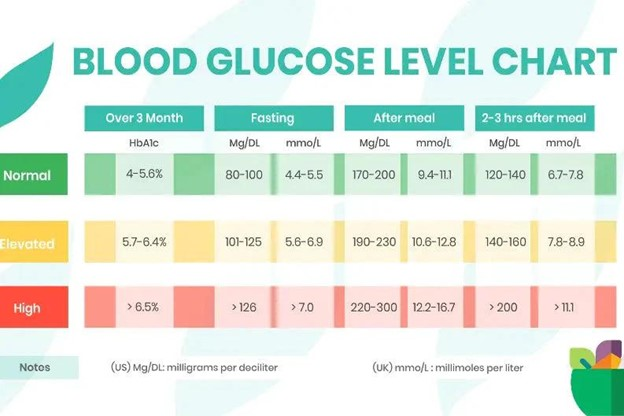
\includegraphics[width=0.5\textwidth]{images/Normal-Blood-Sugar-Levels-Chart.jpg}
    \caption{Blood Glucose levels
    \protect\cite{Agarwal_2025}}
    \label{fig:glucose_chart}
\end{figure}

\subsection{Glycemic Index GI}

An important innovation in the relationship of foods to blood glucose was the introduction of the Glycemic Index by Jenkins et al. \cite{Jenkins_1981}. Glycemic Index (GI) estimates how quickly a standard amount of carbohydrates (50g) is absorbed by the body from a specific food. It measures the speed with which food is absorbed. Measurements require the test subject to fast before eating the food. The amount of food varies according to its carbohydrate content. Blood glucose is then integrated over the next 2 hours. The resulting value is standardized against 50g of pure glucose, yielding a number from 0 (no effect on blood sugar) to 100 (same effect as pure glucose). There are some foods that have GI ratings higher than 100.

\subsection{Glycemic Load GL}

One limitation of GI is that it is difficult to translate into expectations for a given meal. Salmerón et. al. introduced the concept of Glycemic Load (GL) \cite{Salmeron_1997}, which improves upon GI by accounting for the amount of carbohydrates in a 100g serving of the food. In theory, this allows one to calculate a summary metric for any given meal to estimate the effects on blood sugar. In practice, it is a lot of work to weigh each food, look up its GL and then build a GL estimate for the meal. It can be very difficult to find the GL for certain foods. GI and GL also vary when certain foods are mixed \cite{Murillo_2022}

A large number of metrics have been proposed to study glycemic variability (GV). For a comprehensive review see Lazar et al. \cite{Lazar_2023}.

\subsection{Glycemic Increment G+}

With the availability of CGM data, it becomes practical to directly estimate the glycemic response of each meal eaten by the patient. Actual measurements of typical meals can lead to actionable insights into diet.

This paper introduces the concept of Glycemic Increment (G+). G+ directly estimates the blood sugar consequences of particular foods and composite meals (glycemic response). It provides an individualized model of each patient's response to particular foods. The inputs to the model are just a list of foods in a particular meal. The output is a number that directly estimates an increase or decrease in blood sugar over a reasonable period. The model is built without requiring a fasting state or precise measurements of foods. It relies on the "typical serving" used by the patient.

Fig. \ref{fig:gplus_illustrated} shows how G+ is calculated. The left of the chart is the start of a meal. The duration of the chart is the measurement period. The values in blue are the integration of blood glucose values over the measurement period. The orange area, set at the initial blood glucose level, is subtracted from the blue. The difference is divided by the number of hours in the measurement period. The resulting unit is mg-hours/dL.

Standardization to 1 hour allows for the comparison of G+ from different measurement intervals.

Using the starting blood glucose makes it unnecessary for the patient to be fasting at measurement time.

Note that if blood glucose falls significantly below the starting glucose, G+ can yield a negative value. This can happen when a food triggers a rapid insulinic response, causing blood sugar to drop rapidly. For this reason, both very positive and very negative G+ values should be interpreted as a strong glycemic response.

It is not clear whether the low glycemic response is G+ values near zero or G+ values near the mean. Without further examination, the present work assumes the former.

\begin{figure}[tbp]
    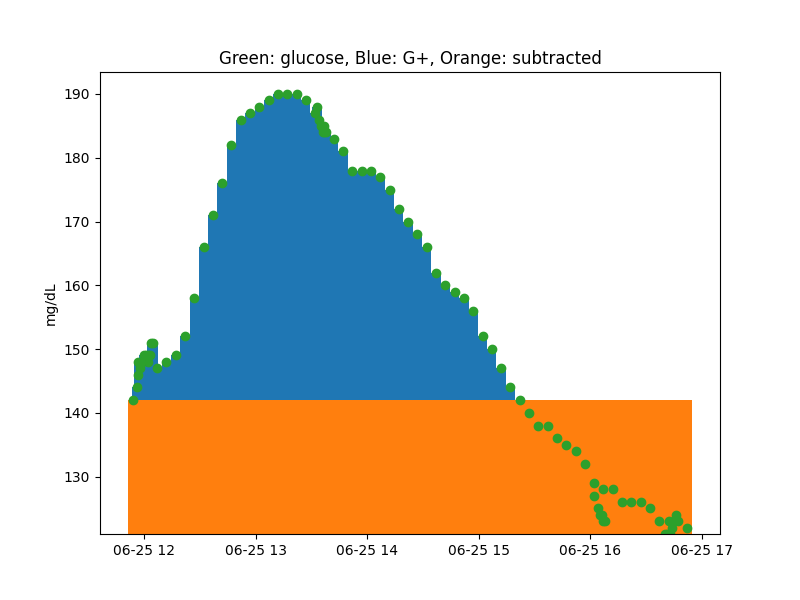
\includegraphics[width=0.5\textwidth]{images/gplus_illustrated.png}
    \caption{Glycemic Increment}
    \label{fig:gplus_illustrated}
\end{figure}

\section{Data}

The data set is 2 years of CGM data taken from the second author. It includes free-form food logs and blood glucose measurements taken every 5 minutes. The data is nearly complete, with only a few gaps related to the periodic challenges associated with acquiring CGM sensors.

The free-form notes have some structure due to consistent commenting by the second author. Foods are comma-separated, and there are additional notations such as restaurants, quantities, and units.

Fig. \ref{fig:glucose_data} shows a sample of raw glucose data.  Fig. \ref{fig:meal_data} shows a sample of raw meal data.

\begin{figure}[tbp]
    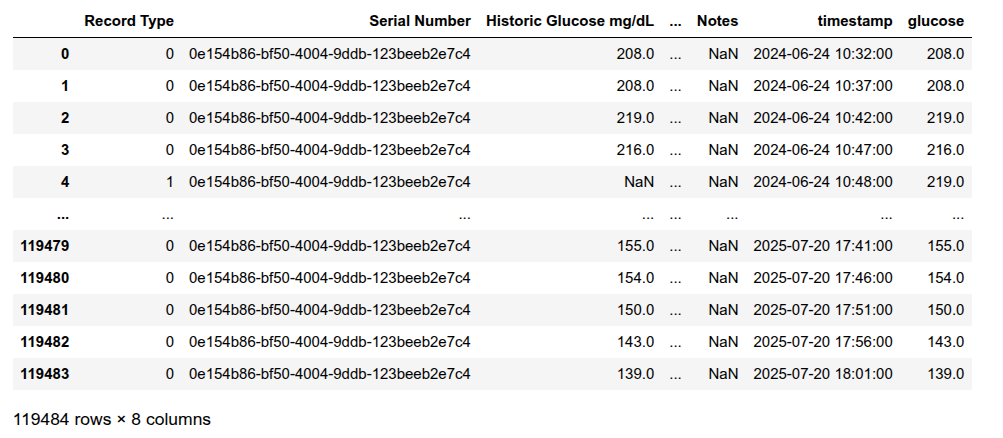
\includegraphics[width=0.5\textwidth]{images/glucose_data.png}
    \caption{Raw Glucose Data}    \label{fig:glucose_data}
\end{figure}

\begin{figure}[htbp]
    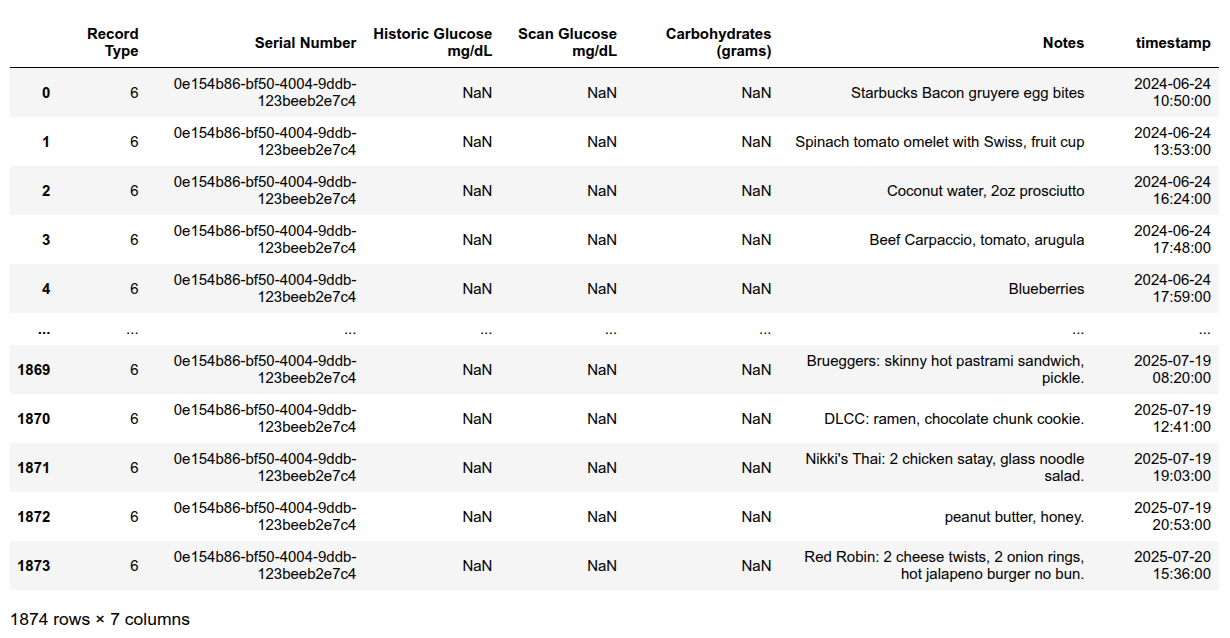
\includegraphics[width=0.5\textwidth]{images/meal_data.png}
    \caption{Raw Meal Data}
    \label{fig:meal_data}
\end{figure}

\section{Methods and Models}

This study defines a regression problem: predict a blood sugar metric based on foods in a meal.

All models use \texttt{sklearn.linea\_model
.LinearRegression} so that the coefficients are interpretable. The coefficient of a food tells how much a serving of that food affects blood sugar.

This study includes models that treat the notes as unstructured and models that account for the semi-structured format used by the second author. The unstructured models are suitable for a patient who might not have recorded foods in the same format. The structured format reports foods more accurately.

The predicted value is Glycemic Increment (G+), introduced for the first time in this study.

\subsection{Meals}

There are three types of meals: \emph{regular}, \emph{extended}, and \emph{unpreceded}.

For \emph{regular} meals, each note in the data set defines a separate meal. The two hours following the note are the measurement period.

For \emph{extended} meals, if a note occurs within 2 hours of another note, it is combined with the preceding note(s). The measurement period starts from the time of the first note to 2 hours after the last note.

If there are no notes for 4 hours before a given note, it is an \emph{unpreceded} meal. The measurement period starts from the time of the note to 30 minutes after.

The three data sets are each split into \emph{train} and \emph{test} sets with \texttt{sklearn.train\_test\_split}, reserving 30\% for the test set.

\subsection{Tokenization and Vectorization}

There are two tokenizers. The generic tokenizer is meant for use by anyone who has been using the notes to record foods that they have eaten. The full format tokenizer is intended for anyone who has been using a specific semi-structured format.

The generic tokenizer is the default tokenizer for \texttt{sklearn.feature\_extraction.CountVectorizer} with unigrams, bigrams, and trigrams. The stop words are \texttt{and}, \texttt{with}, \texttt{servings}, and \texttt{leftovers}.

The full format tokenizer allows each note to start with an optional \emph{restaurant} followed by a colon, and then the remaining string is split on the regular expression \texttt{r'[,;]|and|with'}. This allows foods to be identified by their full name. Each food can start with a quantity and an optional unit. If no quantity is specified, the parser defaults to \texttt{1.0}. The default unit is \texttt{serving}.

There are two vectorizers. The simpler vectorizer is \texttt{CountVectorizer} with binary labels. It is used with the default tokenizer and the full format tokenizer.

The other vectorizer, defined for this study, is \texttt{QuantifierVectorizer} which uses the quantity from the full format parser as the value of the feature. The features themselves are generated by \texttt{CountVectorizer} with the full format vectorizer. It is not possible to use the generic tokenizer with the \texttt{QuantifierVectorizer} as the full format parser is needed to extract quantities from the notes.

\section{Experimental Design and Investigation Strategy}

Each model is presented as a scatter plot of predicted G+ vs. actual G+, with a linear fit line for reference. For a perfect model, the linear fit line would have a slope of \texttt{1.0}.

The plots also include the Pearson Correlation Coefficient (\texttt{1.0} is perfect correlation), and root mean squared error (\texttt{0.0} is a perfect model). The root mean squared error has the same units as the domain (hour-mg/dL), allowing the comparison of error to the coefficients of individual foods.

There are 9 possible models as shown in table \ref{table:models}. There are three meal types, and three possible combinations of vectorizer and tokenizer.

\begin{table}
\centering
\begin{tabular}[tbp]{|l l l|}
    \hline
    meal type   & vectorizer & tokenizer \\
    \hline
    regular     & Binary     & ngrams \\
    regular     & Binary     & full \\
    regular     & Quantifier & full \\
    extended    & Binary     & ngrams \\
    extended    & Binary     & full \\
    extended    & Quantifier & full \\
    unpreceded & Binary     & ngrams \\
    unpreceded & Binary     & full \\
    unpreceded & Quantifier & full \\
    \hline
\end{tabular}
\caption{The 9 models. \label{table:models}}
\end{table}

The \emph{regular} meal type is the simplest interpretation of the data. Every note is a separate meal.

The \emph{extended} meal type attempts to deal with the case when a second set of food has been consumed before the glucose of the preceding food has been fully processed.

The \emph{unpreceded} meal type is an effort to create conditions closer to those used for GI calculation, where the subject is in a state of fasting before testing.

\section{Results and Observations}

Fig. \ref{fig:all_models_tested} shows a variant on calibration curve for each of the models. Here it is used as a continuous approximation of confusion matrix. They horizontal axis is the predicted G+ and the vertical axis is the actual G+. The green line is a best linear fit. The data set for each meal type is a separate test set.

\begin{figure}[tbp]
    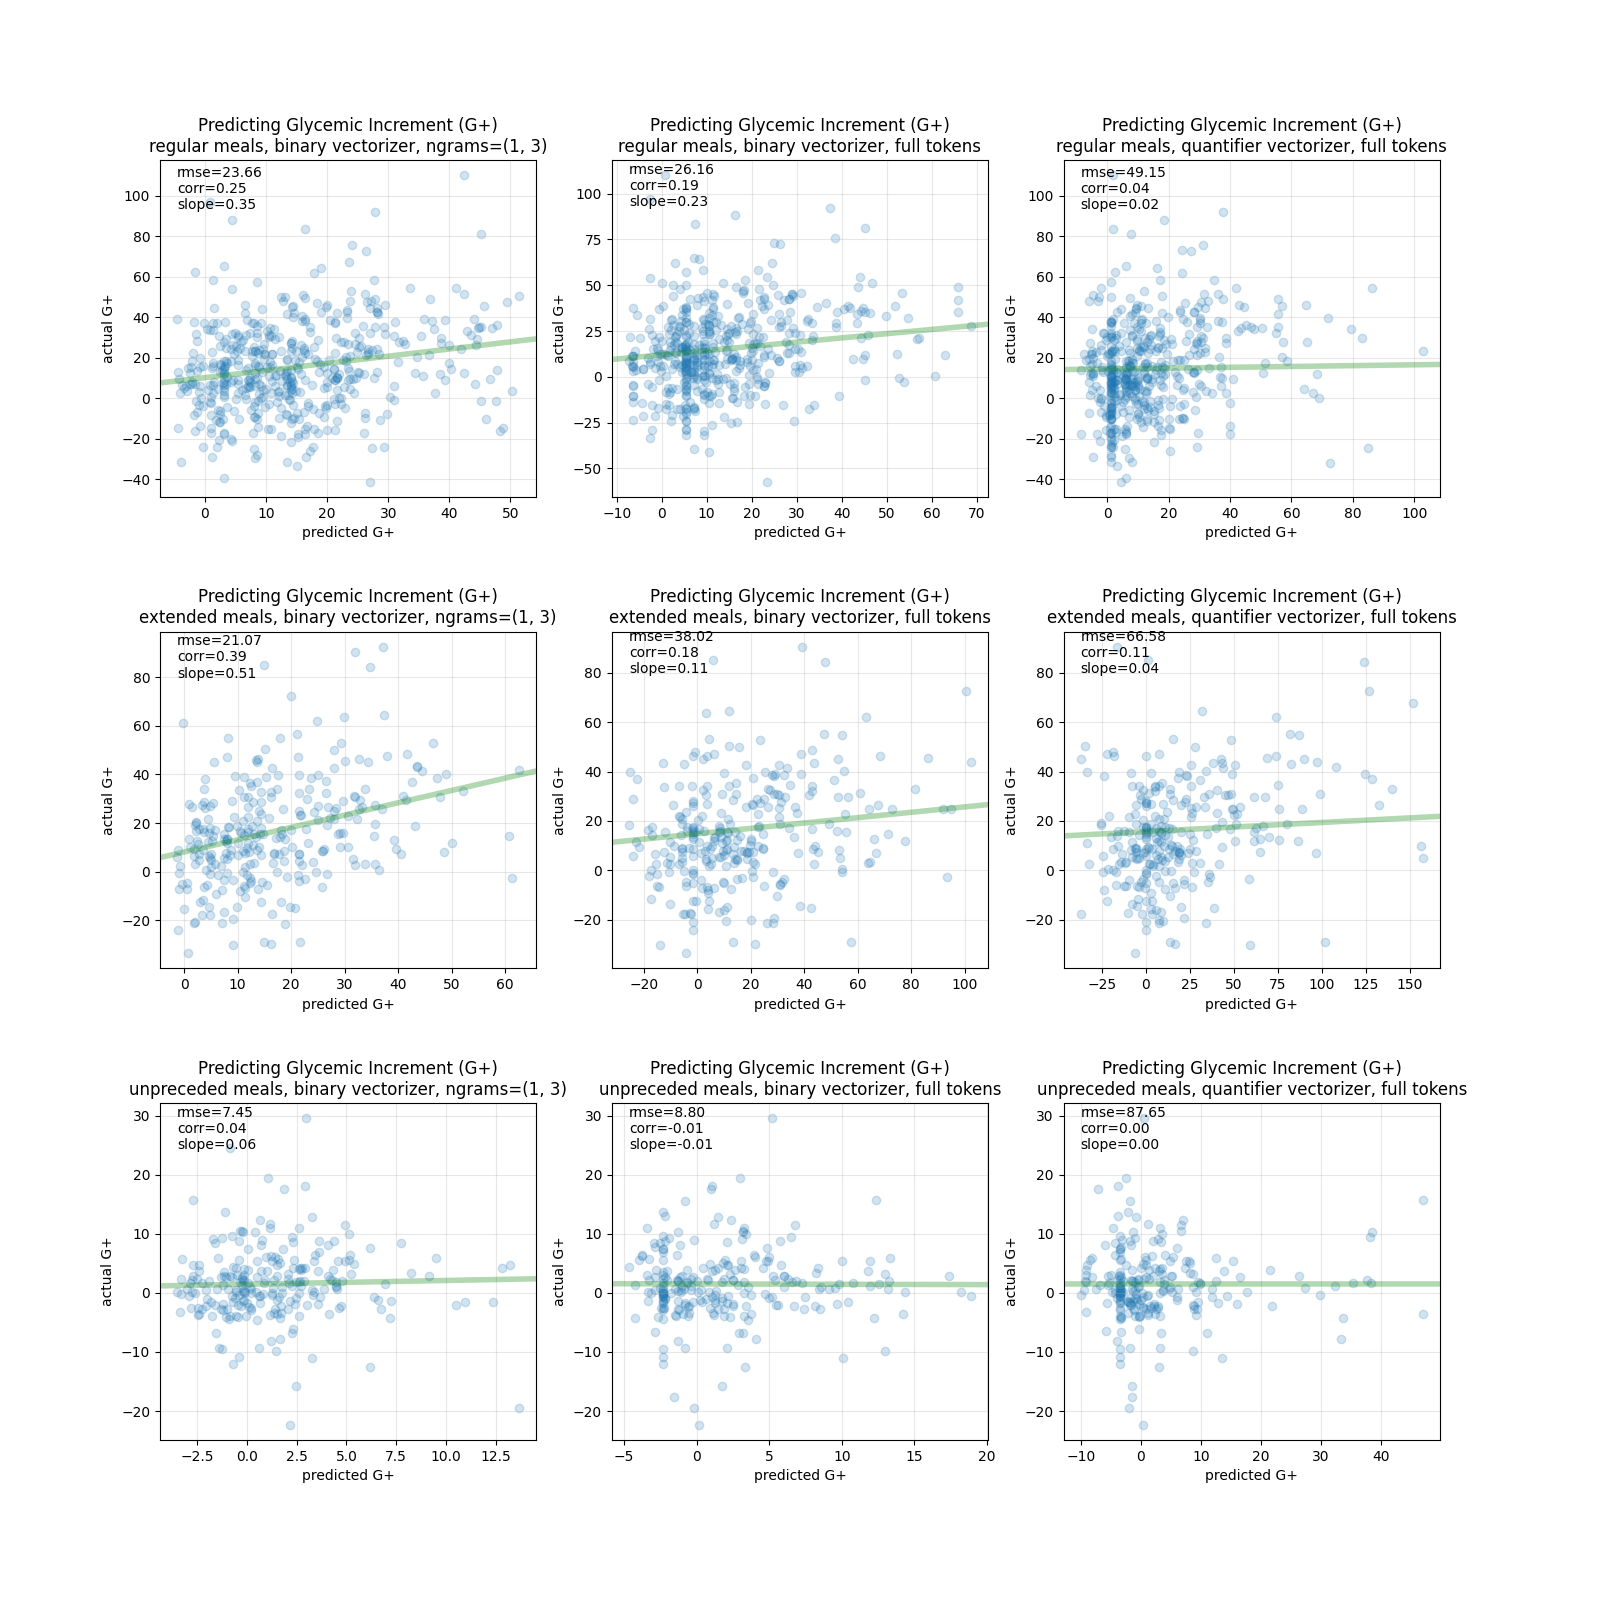
\includegraphics[width=0.5\textwidth]{images/gplus_all_models.png}
    \caption{Model Calibration Plots}
    \label{fig:all_models_tested}
\end{figure}

The three metrics we look at are \emph{root mean squared error} (\emph{rmse}), the correlation coefficient, and the slope of the best linear fit.

The value of \emph{rmse} is in the same units as G+. A perfect model would have an \emph{rmse} of \texttt{0.0}. This metric is most useful for comparing the models.

A perfect model would have a correlation coefficient of \texttt{1.0}. Here it is used as an indicator for the strength of the model.

The slope of the best linear fit shows how well the model approximates the true G+ behavior. A perfect model would have a slope of \texttt{1.0}. A slope near \texttt{0.0} shows a model with no predictive power.

\subsubsection{Calibration Plots}

The three \emph{unpreceded} meal models are worthless. Their correlations and slopes are near \texttt{0}. There is no discernible relationship between the predictions and the actual values.

The three models with the \texttt{QuantifierVectorizer} are similarly terrible. The \emph{extended} meals model has a tiny positive correlation, but it does not appear to have significant predictive power.

The four remaining models appear to be usable. The two full token models have nearly identical correlations (\texttt{0.19} and \texttt{0.18}), and modest slopes.

The two trigram based models (\emph{regular} meals and \emph{extended}) have moderately higher predictive power.

\subsubsection{Food Coefficients}

Figs. \ref{fig:low_best} and \ref{fig:high_best} show the low magnitude and high magnitude food coefficients to confirm that the models make sense. Only the models with reasonable predictive power are in these tables.

Fig. \ref{fig:low_best} shows the foods with the lowest magnitude scores.

The \emph{regular} meals with ngram tokenizer model shows one of the limitations of this tokenizer. All of the small negative values come from a single meal: \texttt{Miracle Noodle, butter, dill, 3 eggs, 8 ciliegine}. Miracle Noodles are a form of konjac, a food with a GI of 0.

The positive values only represent two meals: \texttt{Wendy's: Dave's triple no bun} and \texttt{2 chicken thighs, artichoke, corn with butter, 6 dried apricots. 6 prunes.}

The full tokenizer model holds no surprises. It seems likely that \texttt{braised bed} is a typo for \texttt{braised beef}.

The \emph{extended} meals with ngram tokenizer model holds one surprise. The positive values all come from a combined meal of \texttt{Grilled salmon, salmon skin, salad, black olives, truffle balsamic glaze} and almost an hour later \texttt{2 donuts}. Inexplicably, the donuts appear to have had little effect on blood sugar.

The \texttt{shaking} is from a note unrelated to food, so unsurprisingly did not affect blood sugar.

The \emph{extended} meals with full tokenizer model holds only one surprise, \texttt{Tate's Bake Shop oatmeal raisin cookies}. This food definitely raises blood sugar so it is not clear how it has such a low score. All the other foods make sense. Note that \texttt{hot chocolate milk sweetened} is followed by \texttt{with stevia} in the raw data. The parser treats \texttt{with} as a food separator.

\begin{figure}[tbp]
    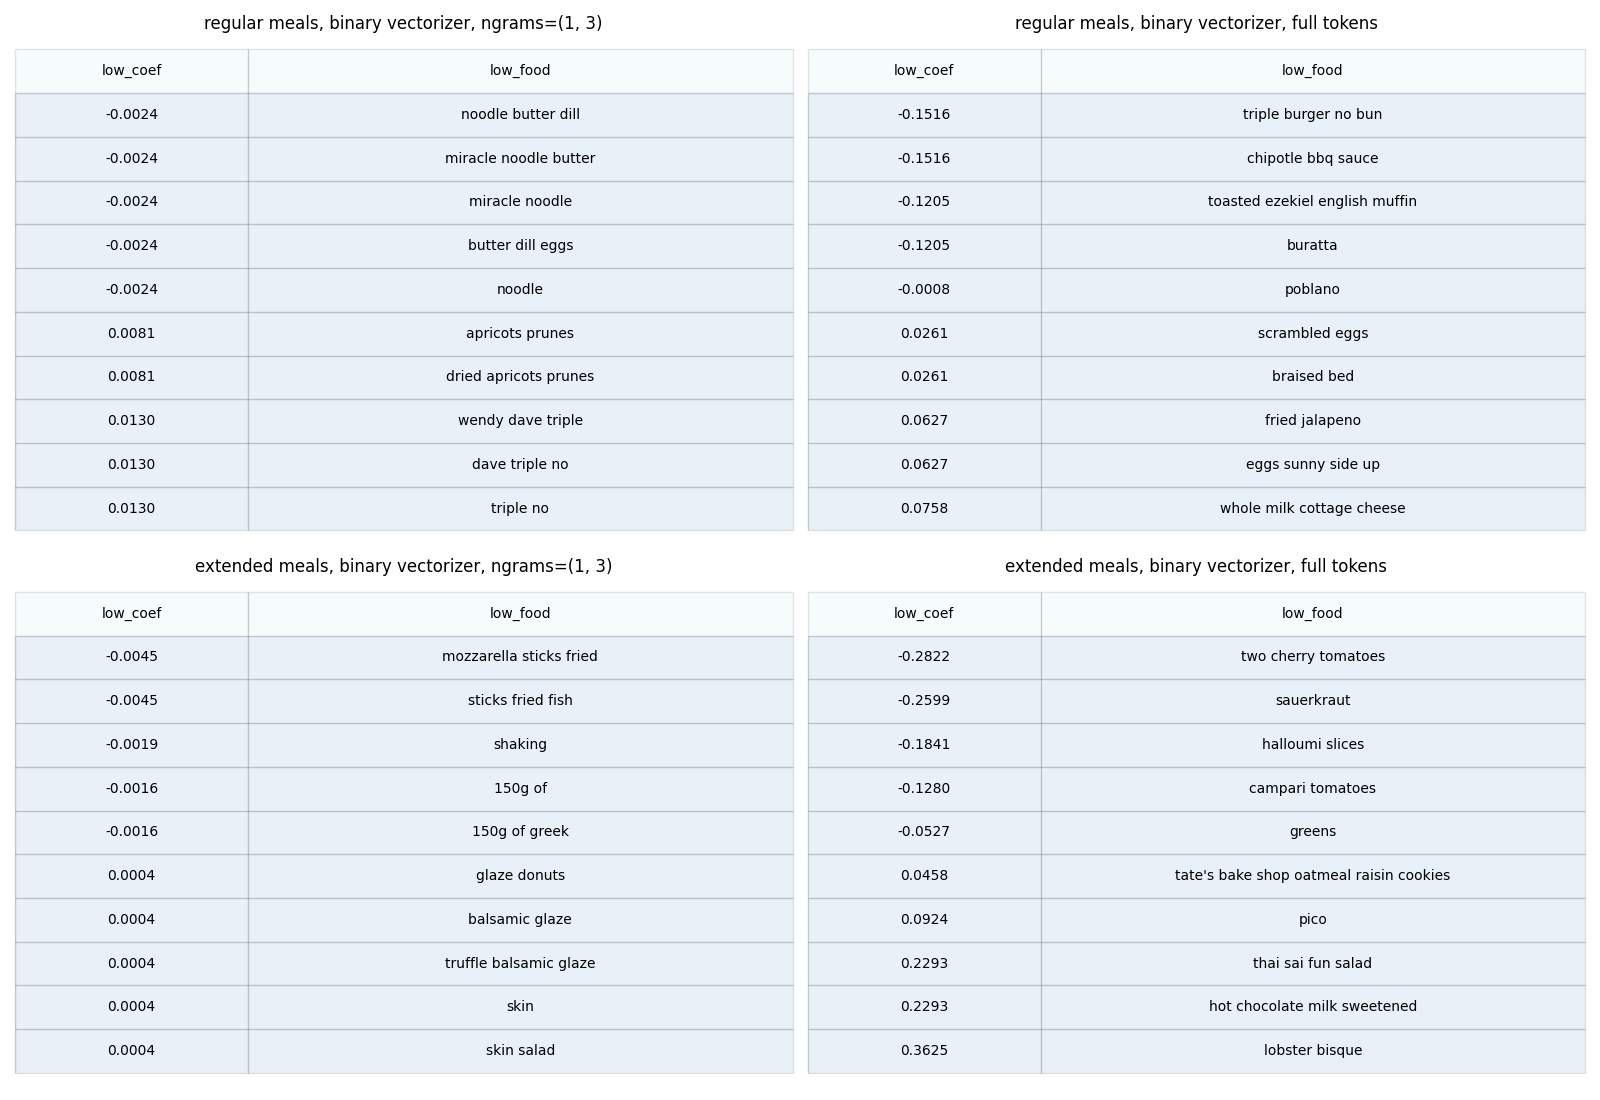
\includegraphics[width=0.5\textwidth]{images/low_gplus_best_models.png}
    \caption{Foods with scores near \texttt{0.0}}
    \label{fig:low_best}
\end{figure}

The high magnitude scores are mostly unsurprising. Eating at Speedway is generally bad for blood sugar. The \texttt{masoor beef} shows another limitation--that food is always eaten with rice, which increases blood sugar.

While not perfect, these models are useful for predicting the effects of specific meals on blood sugar.

\begin{figure}[tbp]
    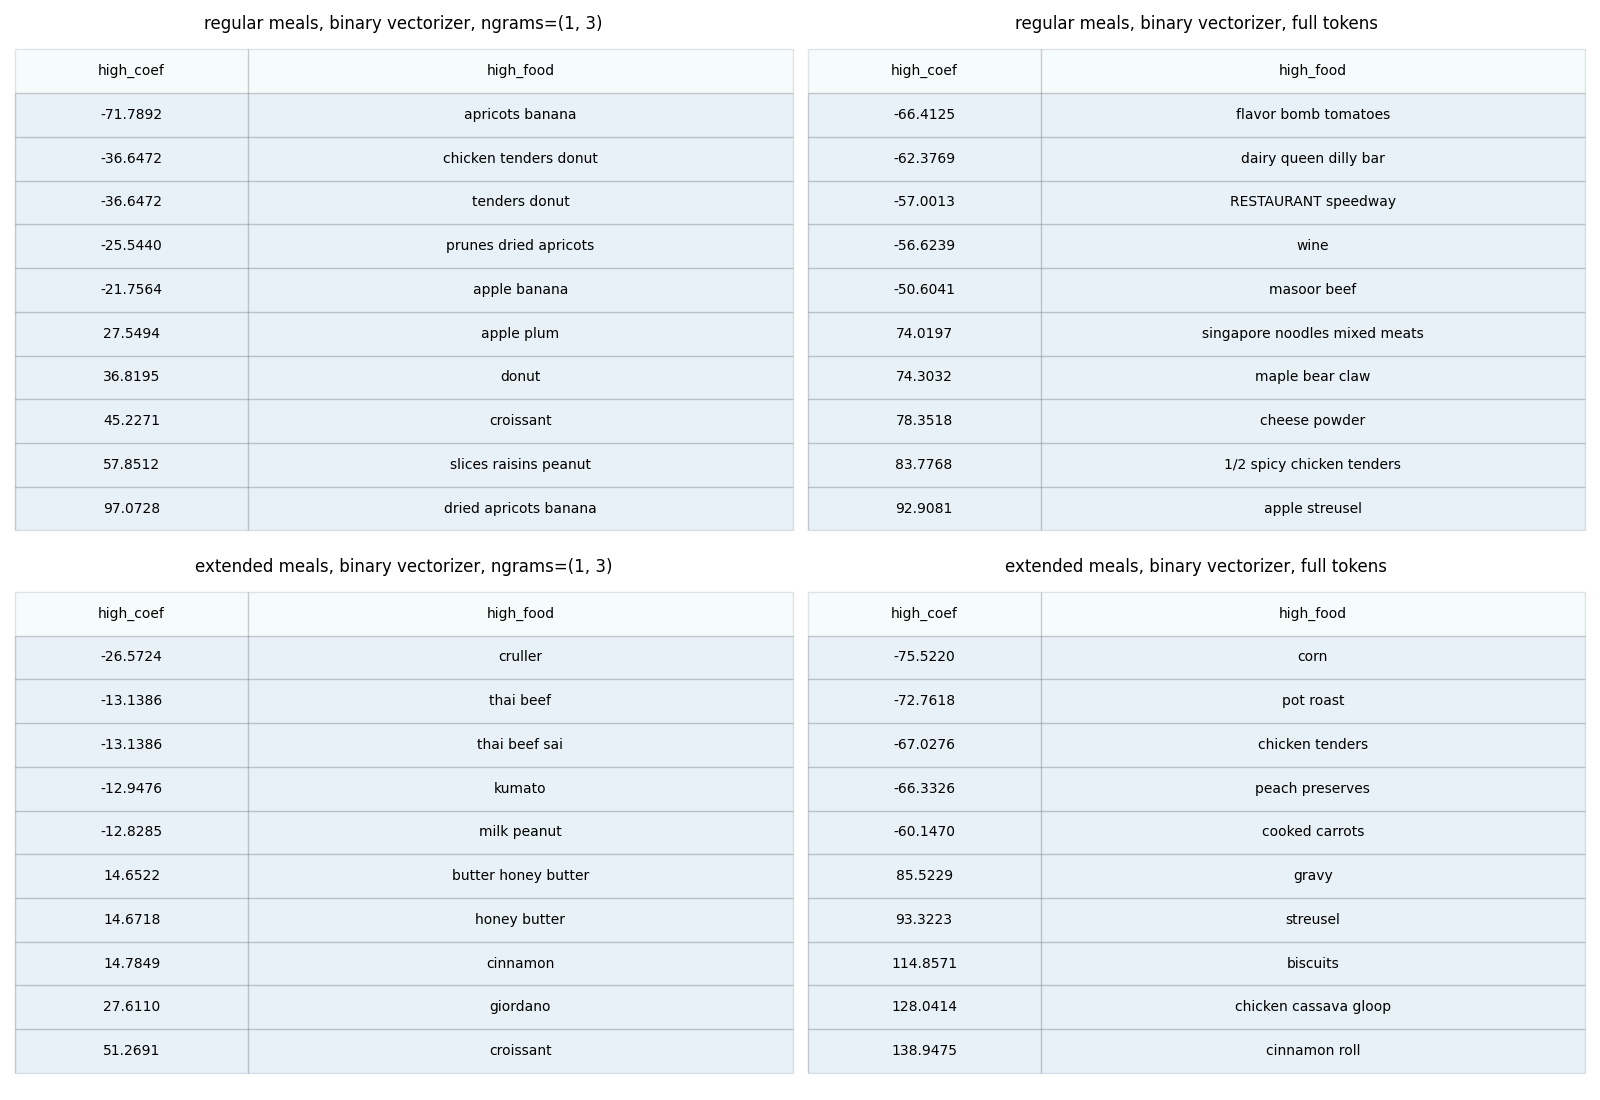
\includegraphics[width=0.5\textwidth]{images/high_gplus_best_models.png}
    \caption{Foods with scores of high magnitude}
    \label{fig:high_best}
\end{figure}

\section{Conclusions}

Individualized medicine is a growing field. The availability of inexpensive sensors that can provide information from activity, blood pressure, blood oxygen, and blood glucose has created a plethora of data.

Patients can use their own data to produce suitable guidance for controlling blood sugar through diet.

The analysis code and data are available via https://github.com/piggyatbaqaqi/sugarbowl.

\section*{Appendix}

\subsection{On negative values}

All 9 models produce negative values for certain foods. Spot-checking shows that these foods are mostly high-GI and high-GL.

Investigation of specific cases suggests three phenomena: insulin reaction, rapid successive meals, and variations in blood sugar not associated with eating.

If a high-GL food is eaten, typically there is a spike in blood sugar followed by a decrease. High-GL foods typically cause rapid rise followed by rapid decrease (hypoglycemia, an insulin reaction).

Some of the foods with negative G + values are often eaten in the hours following the consumption of a high-GL food, so if they have a low-GL, their G+ values will still be negative due to the falling blood glucose from the earlier meal.

The \emph{unpreceded} meals are an effort to isolate only those meals that do not have a predecessor, and therefore have an expectation of stable blood sugar. In fact, blood sugar is not stable for these meals. There are daily variations that do not have an immediate food-related cause.

The \emph{extended} meals are an effort to go the other direction, combining the effects of chained meals, those eaten before the effects of the previous meal have worn off.

The fact that the most negative values are for high-GL foods suggests that the insulin reaction is the dominant effect.

A possible future metric is Absolute G+, in which the absolute difference between the blood sugar measurement and each subsequent measurement is integrated. A food that has no glycemic effect throughout the measurement interval is not the same as a food which has positive and negative effects on blood sugar of equal magnitude. However, both would show G+ of \texttt{0}.

Another area of related modeling would be an attempt to predict the moderating effects of foods on each other. Some form of rule mining could discern when the presence of a given food in a meal causes a lower than expected G+ score.

\subsection{On singletons and rare foods}

An early run of a full token model yielded \texttt{lamb mattar} (lamb with peas sauce) as a very high G+ dish. Although peas are not particularly low-GL, they should not have been considered extreme. A close examination of the data revealed that the one meal of \texttt{lamb mattar} in the data set also includes \texttt{5 servings of diabetic rice}, which is undoubtedly the cause of the high score.

Dealing with rare cases like this remains an open topic of investigation.

\bibliography{glycemic_increment_references}
\bibliographystyle{ieeetr}

\vspace{12pt}

\end{document}
